\section{Configuração do circuito}

A análise de um circuito basicamente é o processo de segmentá-lo em partes menores, sem que haja alteração das suas características de funcionamento, de forma a simplificar seu manuseio.

Alguns conceitos são de fundamental importância para facilitar essa tarefa de análise do circuito, e um destes conceitos é o \textbf{nó}.

O \textbf{nó} é uma \textbf{conexão entre pelo menos três elementos do circuito} ou entre elementos ativos e passivos e é representada por uma circunferência preenchida unindo os terminais dos componentes.

A Figura \ref{fig:CircuitoDesafioNos} mostra em destaque os nós denominados como \textbf{A} e \textbf{B}. As setas nas linhas indicam o sentido da corrente, chegando ou saindo de cada nó.

\begin{figure}[h]
\center
\caption{Nós $A$ e $B$.}
\label{fig:CircuitoDesafioNos}
\subfigure[fig:CircuitoDesafioNoS][Nó superior.]{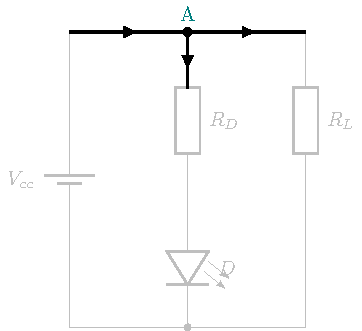
\includegraphics[width=6cm]{fig-circuitoDesafioNoSup}}
\qquad
\subfigure[fig:CircuitoDesafioNoI][Nó inferior.]{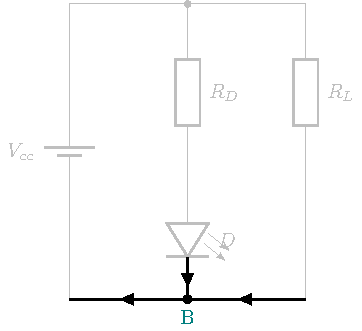
\includegraphics[width=6cm]{fig-circuitoDesafioNoInf}}
\end{figure}




\subsection{Ligação em série}

\textbf{O trecho do circuito entre nós é chamado de ramo. Em um ramo, todos os seus componentes são ligados em série.}
A Figura \ref{fig:CircuitoDesafioRamos} mostra os três ramos ligados aos pontos $A$ e $B$, sendo o ramo central o único que possui mais do que um componente, ou seja, é o único que possui componentes em série. Assim pode-se afirmar que \textbf{ o resistor $R_D$ está em série com o LED $D$}.

\begin{figure}[h]
\center
\caption{Ramos entre os nós $A$ e $B$.}
\label{fig:CircuitoDesafioRamos}
\subfigure[ref1][Ramo com a $Fonte$.]{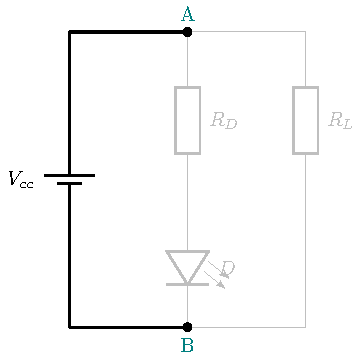
\includegraphics[width=4cm]{fig-circuitoDesafioRamoFonte}}
\qquad
\subfigure[ref2][Ramo com o $R_D$ e $D$.]{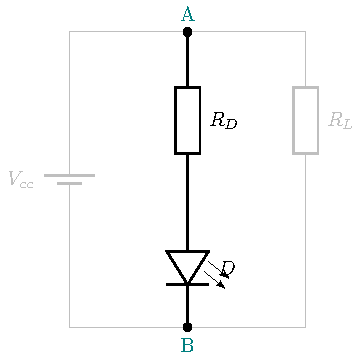
\includegraphics[width=4cm]{fig-circuitoDesafioRamoRLED}}
\qquad
\subfigure[ref3][Ramo com o $R_L$]{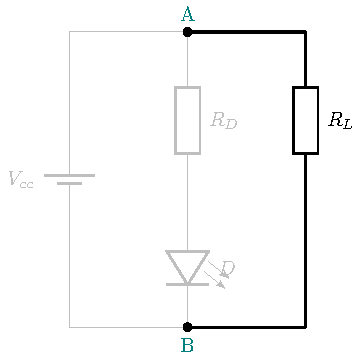
\includegraphics[width=4cm]{fig-circuitoDesafioRamoRL}}
\end{figure}


\subsection{Ligação em paralelo}

O circuito da Figura \ref{fig:CircuitoExemplo} apresenta três nós ($A$, $B$ e $C$) e cinco ramos, cada um contendo apenas um elemento cada ($V_{CC}$, $R_1$, $R_2$, $R_3$ e $R_4$).

\begin{minipage}{\linewidth}
  \centering
  \begin{minipage}{0.45\linewidth}
    Note que \textbf{o nó C aparece duas vezes, mas} não quer dizer que sejam pontos distintos, pelo contrário, \textbf{é o mesmo ponto}, representado em dois lugares. É o ponto de conexão entre os quatro resistores.
  \end{minipage}
  \hspace{0.05\linewidth}
  \begin{minipage}{0.45\linewidth}
    \begin{figure}[H]
      \centering
      \caption{Nós do circuito.}
      \label{fig:CircuitoExemplo}
      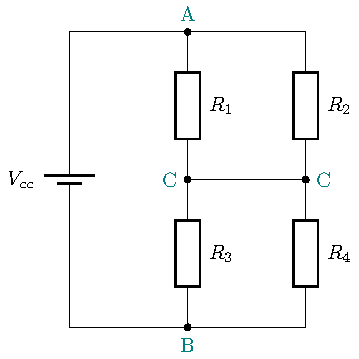
\includegraphics[scale=1.0]{fig-circuitoExemplo}
%
%      {\small Fonte: Próprio autor.}
    \end{figure}
  \end{minipage}
\end{minipage}

Como existem dois ramos ligados aos \textbf{mesmos nós}, isso significa que seus elementos \textbf{estão em paralelo}. Como em cada ramo só existe um resistor, então:

\begin{itemize}
  \item $R_1$ é paralelo ao $R_2$
  \item $R_3$ é paralelo ao $R_4$
\end{itemize}

Nesse circuito, nenhum ramo apresenta mais do que um elemento, assim não há componentes em série.
